\documentclass[10pt]{ltjsarticle}
\usepackage{amsmath}
\usepackage{booktabs}
\usepackage{graphicx}
\usepackage[margin=17mm]{geometry}
\usepackage{hyperref}
\usepackage{enumitem}
\hypersetup{colorlinks=true,urlcolor=blue,linkcolor=black}
\setlist[itemize]{leftmargin=1.6em,itemsep=0.15em,topsep=0.25em}
\setlength{\parskip}{0.25em}
\setlength{\parindent}{1em}

\newcommand{\StudentName}{広野　翔}
\newcommand{\StudentID}{265t355t}
\newcommand{\RepositoryURL}{https://github.com/shoH1895/kobe-u-265t355t-final_assignment}

\title{学食メニュー栄養管理・食事提案アプリ}
\author{\StudentName\quad（\StudentID）}
\date{2026年8月}

\begin{document}
\maketitle
\vspace{-2.0em}
\begin{center}
GitHubリポジトリ：\url{\RepositoryURL}
\end{center}
\vspace{-0.5em}

\section{ソフトウェアの目的}
本ソフトウェアは，神戸大学生協LANS BOX食堂のWebサイトから起動時に当日のメニュー名，価格，栄養価を取得し，食事選びを支援するものである．起動直後に昼食を食べたかを選択し，昼食前には「その日のおすすめメニュー」を必ず含み，指定価格帯を満たす組み合わせを提示する．昼食後には実際に食べた料理を入力し，1日の目標量から不足分を計算して夕食候補を提示する．利用者は価格だけでなく，エネルギー，たんぱく質，脂質，炭水化物，食塩，カルシウム，野菜量，鉄を同時に比較できる．なお，本アプリは食事選びの参考情報を示すものであり，医療・栄養指導を目的としない．

\section{実装上の工夫}
Web取得，最適化，画面表示，可視化を別モジュールに分割し，処理を追いやすくした．主な工夫は以下の通りである．
\begin{itemize}
  \item \texttt{requests}とBeautifulSoupでHTMLを解析し，取得できない場合はPlaywright，前回キャッシュ，予備CSVの順に切り替える．
  \item Web取得データと常設メニューを\texttt{pandas.DataFrame}へ統一する．同名商品はWeb側を優先し，ライス，味噌汁，通年・夏季の麺類を補完する．
  \item 昼食探索ではおすすめ料理を固定し，追加料理の組み合わせを全探索する．主菜には主食を必須とし，丼・麺類には別の主食を追加しないため，実際の食事として不自然な候補を除外する．
  \item 栄養評価には，目標値で無次元化した重み付き二乗誤差
  \[
    S=\sum_i w_i\left(\frac{x_i-t_i}{t_i}\right)^2
  \]
  を用いる．脂質と食塩は目標超過時の係数を大きくし，過剰摂取を強く減点する．
  \item Streamlitで入力画面を作り，Matplotlibで達成率を表示する．図はPDFとして保存でき，ベクター形式のままレポート等へ利用できる．
\end{itemize}

\section{有用性と完成度の検証}
2026年8月4日の予備データと常設メニューを用い，昼食目標を1日目標の35\%，最低価格を400円に固定し，上限価格を500--700円の範囲で50円ずつ変更して検証した．おすすめ料理は「豚肉の生姜焼き」に固定し，各上限価格で評価値$S$が最小となる組み合わせを求めた．評価値は小さいほど昼食目標に近く，栄養面での適合度が高いことを表す．

\begin{center}
\small
\begin{tabular}{@{}cp{73mm}rrr@{}}
\toprule
上限 & 提案された組み合わせ & 実価格 & 余裕 & 評価値$S$ \\
\midrule
500円 & 豚肉の生姜焼き＋ライス（小） & 484円 & 16円 & 2.048 \\
700円 & 豚肉の生姜焼き＋ライス（中）＋蒸し鶏オクラ和風和え & 627円 & 73円 & 1.341 \\
\bottomrule
\end{tabular}
\end{center}

上限500円では主菜とライス（小）の組み合わせが選ばれたが，上限を600円以上にすると副菜を追加でき，エネルギー，炭水化物，野菜量などの不足を補えるようになった．上限500円から650円へ広げると評価値は2.048から1.341へ34.5\%改善した．一方，650円と700円では同じ627円の組み合わせが選ばれ，評価値も変化しなかった．そのため，上限700円では73円の余裕が残り，価格上限を高く設定しても必ず上限まで支出するわけではないことが分かる．図\ref{fig:verification}から，予算を増やすほど栄養面は改善する一方，650円付近から改善が飽和することを確認できる．利用者は上限価格を変更し，栄養面の改善量と追加費用，残る予算の関係を比較して，自身が納得できる価格帯を選択できる．

\begin{figure}[htbp]
  \centering
  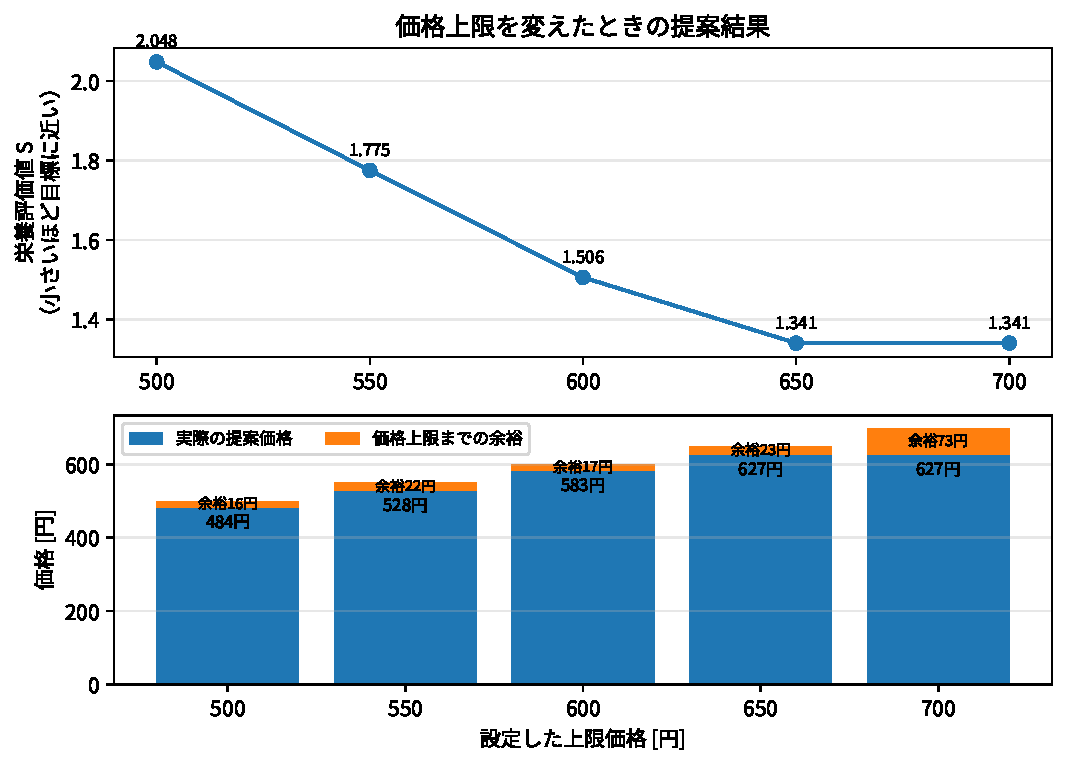
\includegraphics[width=0.86\linewidth]{price_range_verification.pdf}
  \caption{上限価格と栄養評価値・予算余裕の関係（Matplotlibで作成したPDF）}
  \label{fig:verification}
\end{figure}

さらに，単体テストを実行し，主菜候補へ必ず主食が含まれること，価格帯とおすすめ料理の条件を満たすこと，HTMLから料理名・価格・カテゴリを正しく取得すること，夏季のみ冷やし麺を追加することを検証した．GitHub ActionsではpushおよびPull Requestごとに型チェックとテストを自動実行するため，変更による機能破壊も検出できる．

\section{AIの使用}
OpenAIのChatGPT（GPT-5.6 Thinking）を，設計案，コードの初稿，テスト項目，READMEおよびレポート草案の作成に使用した．使用時は，まず必要機能をフローチャートへ分解し，その後にモジュール単位で生成させた．また，実行画面を確認して「料理名が店舗名になる」「カテゴリがすべて副菜になる」「主菜にライスが付かない」「グラフが文字化けする」といった具体的な不具合を提示し，原因箇所と再現条件を限定して修正した．生成結果をそのまま提出せず，授業で扱ったpandas，Matplotlib，型ヒント，pytest，GitHub Actionsの範囲で読解・修正できる構成へ整理した点が，AI利用上の工夫である．

\end{document}
